\section{ueaclib.h File Reference}
\label{ueaclib_8h}\index{ueaclib.h@{ueaclib.h}}


This graph shows which files directly or indirectly include this file:\begin{figure}[H]
\begin{center}
\leavevmode
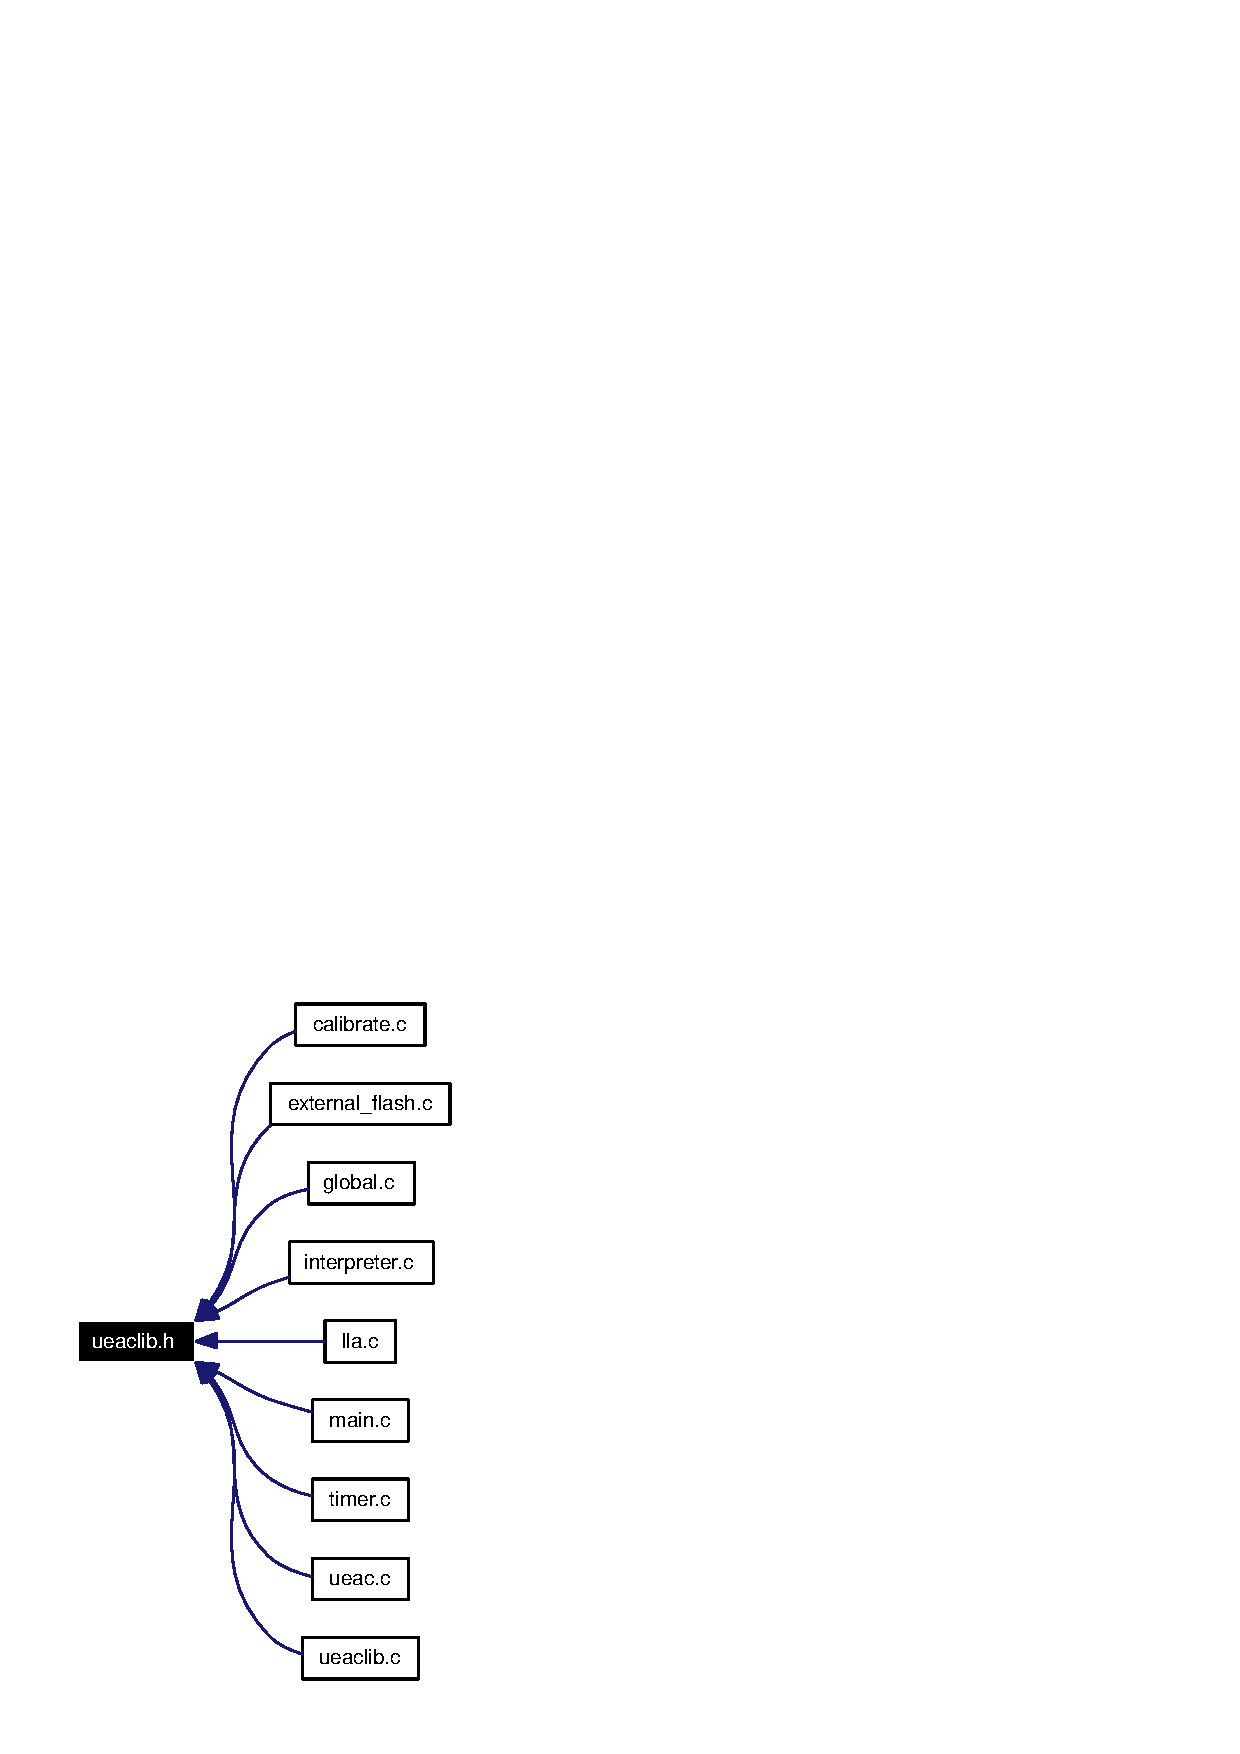
\includegraphics[width=108pt]{ueaclib_8h__dep__incl}
\end{center}
\end{figure}
\subsection*{Defines}
\begin{CompactItemize}
\item 
\#define {\bf BLACK}~\char`\"{}$\backslash$x1B[30m\char`\"{}
\item 
\#define {\bf RED}~\char`\"{}$\backslash$x1B[31m\char`\"{}
\item 
\#define {\bf GREEN}~\char`\"{}$\backslash$x1B[32m\char`\"{}
\item 
\#define {\bf BACK\_\-WHITE}~\char`\"{}$\backslash$x1B[47m\char`\"{}
\item 
\#define {\bf CLR}~\char`\"{}$\backslash$033[2J\char`\"{}
\item 
\#define {\bf TERM\_\-RESET}~\char`\"{}$\backslash$033[H\char`\"{}
\end{CompactItemize}
\subsection*{Functions}
\begin{CompactItemize}
\item 
void {\bf init\_\-sys} (void)
\item 
int {\bf putchar\_\-0} (int)
\item 
char {\bf getchar\_\-0} (void)
\item 
int {\bf putchar} (int)
\item 
char {\bf getchar} (void)
\item 
unsigned char {\bf send\_\-spi\_\-byte} (unsigned char)
\item 
void {\bf write\_\-dac} (int, int)
\item 
void {\bf write\_\-current} (int, int)
\item 
void {\bf write\_\-led} (int, int)
\item 
void {\bf write\_\-lla} (int, int)
\item 
void {\bf start\_\-a2d\_\-converter} (void)
\item 
int {\bf wait\_\-a2d\_\-busy} (void)
\item 
void {\bf write\_\-analog\_\-mux} (unsigned char)
\item 
void {\bf system\_\-reset} (void)
\item 
void {\bf led\_\-pwm} (int)
\item 
void {\bf clear\_\-led\_\-screen} (void)
\end{CompactItemize}


\subsection{Define Documentation}
\index{ueaclib.h@{ueaclib.h}!BACK_WHITE@{BACK\_\-WHITE}}
\index{BACK_WHITE@{BACK\_\-WHITE}!ueaclib.h@{ueaclib.h}}
\subsubsection{\setlength{\rightskip}{0pt plus 5cm}\#define BACK\_\-WHITE~\char`\"{}$\backslash$x1B[47m\char`\"{}}\label{ueaclib_8h_a3}




Definition at line 68 of file ueaclib.h.

Referenced by main().\index{ueaclib.h@{ueaclib.h}!BLACK@{BLACK}}
\index{BLACK@{BLACK}!ueaclib.h@{ueaclib.h}}
\subsubsection{\setlength{\rightskip}{0pt plus 5cm}\#define BLACK~\char`\"{}$\backslash$x1B[30m\char`\"{}}\label{ueaclib_8h_a0}




Definition at line 65 of file ueaclib.h.

Referenced by flash\_\-integrity\_\-test(), and scan\_\-leds().\index{ueaclib.h@{ueaclib.h}!CLR@{CLR}}
\index{CLR@{CLR}!ueaclib.h@{ueaclib.h}}
\subsubsection{\setlength{\rightskip}{0pt plus 5cm}\#define CLR~\char`\"{}$\backslash$033[2J\char`\"{}}\label{ueaclib_8h_a4}




Definition at line 70 of file ueaclib.h.

Referenced by main().\index{ueaclib.h@{ueaclib.h}!GREEN@{GREEN}}
\index{GREEN@{GREEN}!ueaclib.h@{ueaclib.h}}
\subsubsection{\setlength{\rightskip}{0pt plus 5cm}\#define GREEN~\char`\"{}$\backslash$x1B[32m\char`\"{}}\label{ueaclib_8h_a2}




Definition at line 67 of file ueaclib.h.

Referenced by flash\_\-integrity\_\-test(), and scan\_\-leds().\index{ueaclib.h@{ueaclib.h}!RED@{RED}}
\index{RED@{RED}!ueaclib.h@{ueaclib.h}}
\subsubsection{\setlength{\rightskip}{0pt plus 5cm}\#define RED~\char`\"{}$\backslash$x1B[31m\char`\"{}}\label{ueaclib_8h_a1}




Definition at line 66 of file ueaclib.h.

Referenced by flash\_\-integrity\_\-test().\index{ueaclib.h@{ueaclib.h}!TERM_RESET@{TERM\_\-RESET}}
\index{TERM_RESET@{TERM\_\-RESET}!ueaclib.h@{ueaclib.h}}
\subsubsection{\setlength{\rightskip}{0pt plus 5cm}\#define TERM\_\-RESET~\char`\"{}$\backslash$033[H\char`\"{}}\label{ueaclib_8h_a5}




Definition at line 71 of file ueaclib.h.

\subsection{Function Documentation}
\index{ueaclib.h@{ueaclib.h}!clear_led_screen@{clear\_\-led\_\-screen}}
\index{clear_led_screen@{clear\_\-led\_\-screen}!ueaclib.h@{ueaclib.h}}
\subsubsection{\setlength{\rightskip}{0pt plus 5cm}void clear\_\-led\_\-screen (void)}\label{ueaclib_8h_a21}




Definition at line 489 of file ueaclib.c.

Referenced by ueac\_\-execute\_\-instruction().

\footnotesize\begin{verbatim}489                              {
490   P1OUT=0;
491   P5OUT=0x07;
492   P5OUT=0;
493   P2OUT&=~0x01;
494 }
\end{verbatim}\normalsize 


\index{ueaclib.h@{ueaclib.h}!getchar@{getchar}}
\index{getchar@{getchar}!ueaclib.h@{ueaclib.h}}
\subsubsection{\setlength{\rightskip}{0pt plus 5cm}char getchar (void)}\label{ueaclib_8h_a10}




Definition at line 184 of file ueaclib.c.

Referenced by current\_\-output\_\-calibration(), and get\_\-command().

\footnotesize\begin{verbatim}184                    {
185   char rx_data;
186   while (!(IFG2&URXIFG1));
187   rx_data= RXBUF1;
188   return (rx_data);
189 }
\end{verbatim}\normalsize 


\index{ueaclib.h@{ueaclib.h}!getchar_0@{getchar\_\-0}}
\index{getchar_0@{getchar\_\-0}!ueaclib.h@{ueaclib.h}}
\subsubsection{\setlength{\rightskip}{0pt plus 5cm}char getchar\_\-0 (void)}\label{ueaclib_8h_a8}


\index{ueaclib.h@{ueaclib.h}!init_sys@{init\_\-sys}}
\index{init_sys@{init\_\-sys}!ueaclib.h@{ueaclib.h}}
\subsubsection{\setlength{\rightskip}{0pt plus 5cm}void init\_\-sys (void)}\label{ueaclib_8h_a6}




Definition at line 79 of file ueaclib.c.

References clear\_\-latches(), init\_\-a2d(), init\_\-dac(), init\_\-pins(), init\_\-serial\_\-1(), init\_\-spi\_\-0(), init\_\-timer\_\-a(), and Set\_\-DCO().

Referenced by main().

\footnotesize\begin{verbatim}79                     {
80   unsigned int i;
81   WDTCTL = WDTPW + WDTHOLD;    // Stop watchdog
82   init_pins();                 // Setup the discrete I/O - important to enable 8Mhz crystal 
83   for (i = 0xFFFF;i>0;i--);    // Delay for XTAL and oscillator to fire up and settle
84   Set_DCO();                   // calibrate DCO using the 32.768Khz crystal to 3.686400 Mhz  
85   init_spi_0();
86   init_serial_1();             // initialize USB virtual serial port
87   init_timer_a();              
88   init_dac();
89   init_a2d();
90   clear_latches();
91   _EINT();                     // Global interrupt enable
92 }
\end{verbatim}\normalsize 




Here is the call graph for this function:\begin{figure}[H]
\begin{center}
\leavevmode
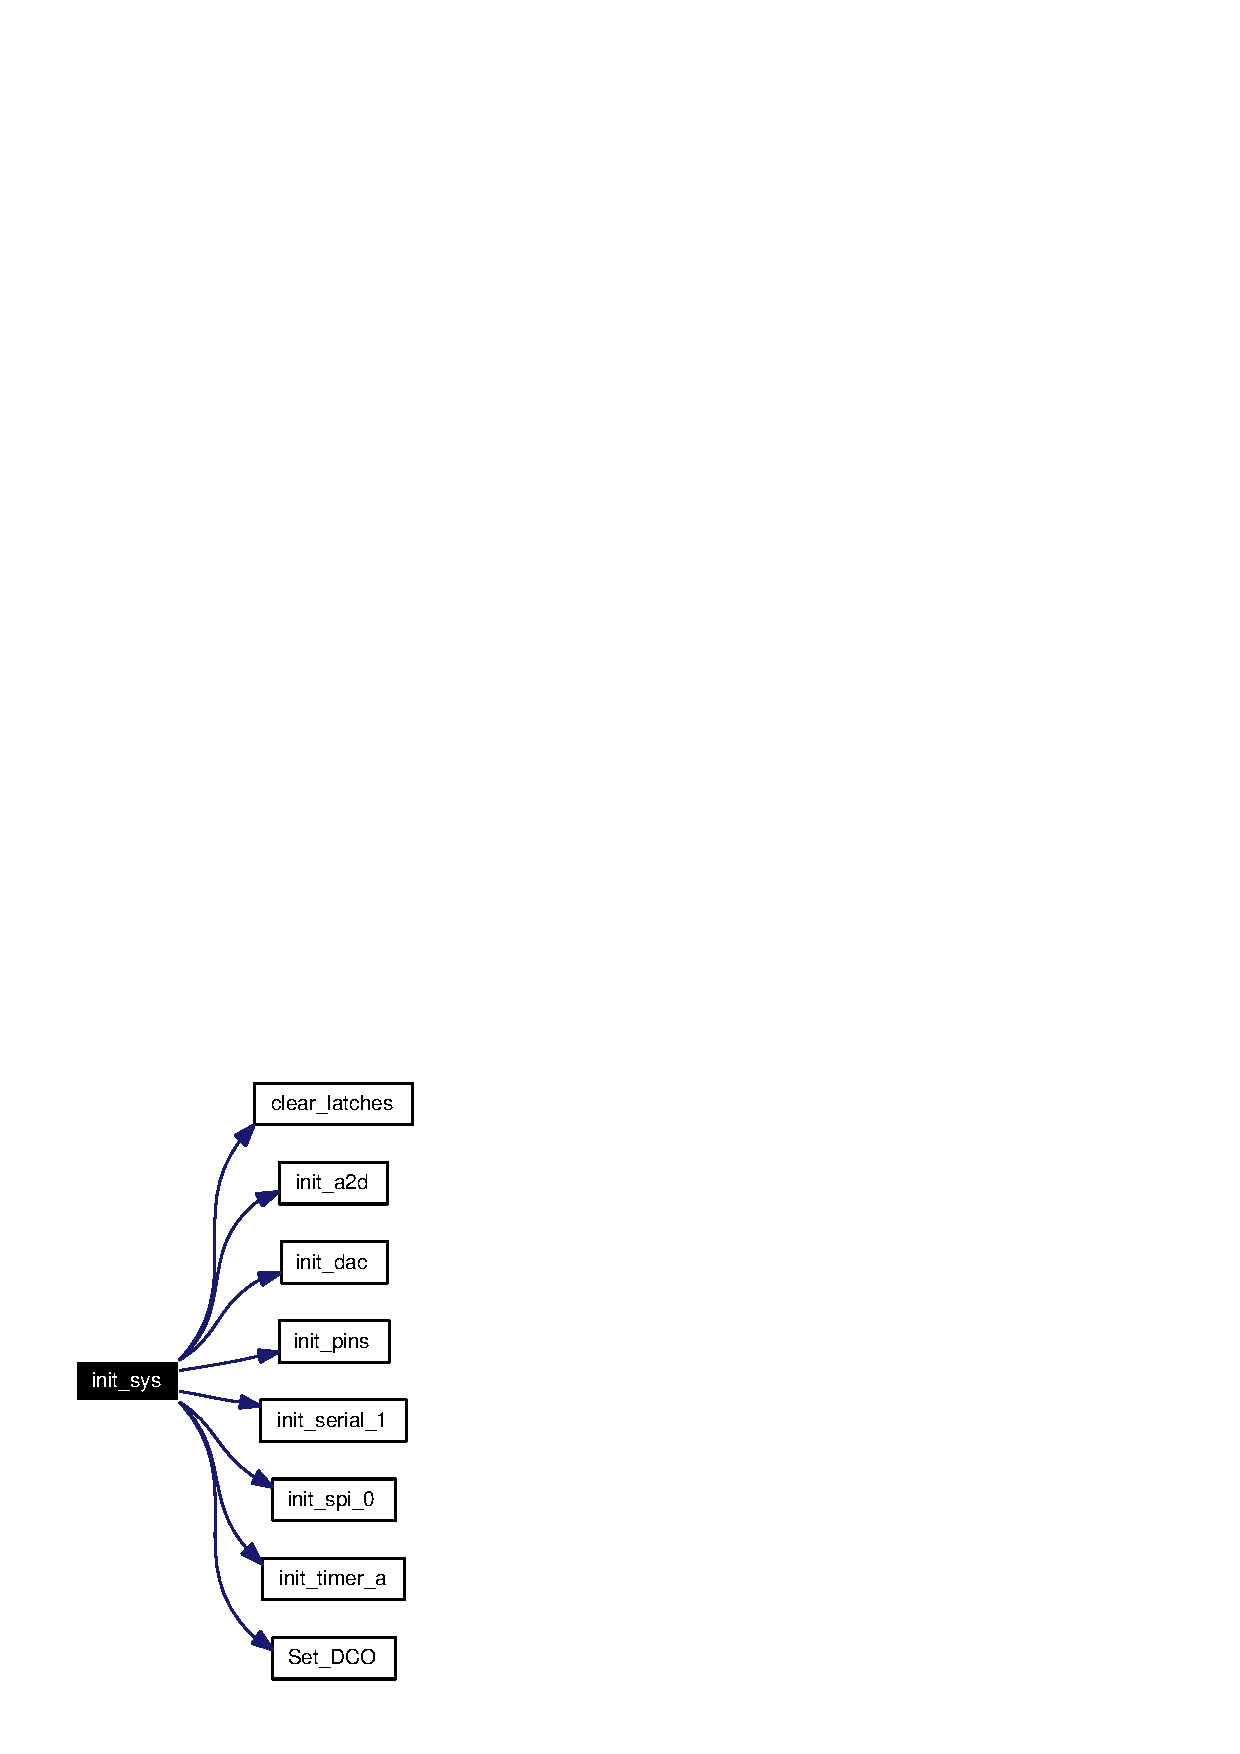
\includegraphics[width=99pt]{ueaclib_8h_a6_cgraph}
\end{center}
\end{figure}
\index{ueaclib.h@{ueaclib.h}!led_pwm@{led\_\-pwm}}
\index{led_pwm@{led\_\-pwm}!ueaclib.h@{ueaclib.h}}
\subsubsection{\setlength{\rightskip}{0pt plus 5cm}void led\_\-pwm (int)}\label{ueaclib_8h_a20}




Definition at line 441 of file ueaclib.c.

References high\_\-time\_\-limit, and PWM\_\-COUNT\_\-MASK.

Referenced by timer\_\-a0\_\-irq().

\footnotesize\begin{verbatim}441                           {
442   static unsigned char counter=0;
443   if (enable) {
444     counter++;
445     counter&=PWM_COUNT_MASK; 
446     if (!counter) {
447       P1OUT=0xFF;
448       P5OUT=0x07;
449       P5OUT=0;
450       P2OUT|=0x01;
451     }
452     P1OUT=0xFF;
453     if (counter>=high_time_limit[0]) P1OUT&=~0x01;
454     if (counter>=high_time_limit[1]) P1OUT&=~0x02;
455     if (counter>=high_time_limit[2]) P1OUT&=~0x04;
456     if (counter>=high_time_limit[3]) P1OUT&=~0x08;
457     if (counter>=high_time_limit[4]) P1OUT&=~0x10;
458     if (counter>=high_time_limit[5]) P1OUT&=~0x20;
459     if (counter>=high_time_limit[6]) P1OUT&=~0x40;
460     if (counter>=high_time_limit[7]) P1OUT&=~0x80;
461     P5OUT=0x01;
462     P5OUT=0x00;
463     P1OUT=0xFF;
464     if (counter>=high_time_limit[8]) P1OUT&=~0x01;
465     if (counter>=high_time_limit[9]) P1OUT&=~0x02;
466     if (counter>=high_time_limit[10]) P1OUT&=~0x04;
467     if (counter>=high_time_limit[11]) P1OUT&=~0x08;
468     if (counter>=high_time_limit[12]) P1OUT&=~0x10;
469     if (counter>=high_time_limit[13]) P1OUT&=~0x20;
470     if (counter>=high_time_limit[14]) P1OUT&=~0x40;
471     if (counter>=high_time_limit[15]) P1OUT&=~0x80;
472     P5OUT=0x02;
473     P5OUT=0x00;
474     P1OUT=0xFF;
475     if (counter>=high_time_limit[16]) P1OUT&=~0x01;
476     if (counter>=high_time_limit[17]) P1OUT&=~0x02;
477     if (counter>=high_time_limit[18]) P1OUT&=~0x04;
478     if (counter>=high_time_limit[19]) P1OUT&=~0x08;
479     if (counter>=high_time_limit[20]) P1OUT&=~0x10;
480     if (counter>=high_time_limit[21]) P1OUT&=~0x20;
481     if (counter>=high_time_limit[22]) P1OUT&=~0x40;
482     if (counter>=high_time_limit[23]) P1OUT&=~0x80;
483     P5OUT=0x04;
484     P5OUT=0x00;
485     if (counter>=high_time_limit[24]) P2OUT&=~0x01;
486   }
487 }
\end{verbatim}\normalsize 


\index{ueaclib.h@{ueaclib.h}!putchar@{putchar}}
\index{putchar@{putchar}!ueaclib.h@{ueaclib.h}}
\subsubsection{\setlength{\rightskip}{0pt plus 5cm}int putchar (int)}\label{ueaclib_8h_a9}




Definition at line 178 of file ueaclib.c.

\footnotesize\begin{verbatim}178                         {
179   while (!(IFG2&UTXIFG1));
180   TXBUF1=in_char;
181   return(0);
182 }
\end{verbatim}\normalsize 


\index{ueaclib.h@{ueaclib.h}!putchar_0@{putchar\_\-0}}
\index{putchar_0@{putchar\_\-0}!ueaclib.h@{ueaclib.h}}
\subsubsection{\setlength{\rightskip}{0pt plus 5cm}int putchar\_\-0 (int)}\label{ueaclib_8h_a7}


\index{ueaclib.h@{ueaclib.h}!send_spi_byte@{send\_\-spi\_\-byte}}
\index{send_spi_byte@{send\_\-spi\_\-byte}!ueaclib.h@{ueaclib.h}}
\subsubsection{\setlength{\rightskip}{0pt plus 5cm}unsigned char send\_\-spi\_\-byte (unsigned {\em char})}\label{ueaclib_8h_a11}




Definition at line 154 of file ueaclib.c.

\footnotesize\begin{verbatim}154                                                      {
155   TXBUF0 = data_byte;        // buffer 1 write  
156   while(!(UTCTL0&0x01));     // wait until transmitter empty
157   return(RXBUF0);            // return any received data
158                              // No data returned from DAC
159                              // SPI flash returns read data
160 }
\end{verbatim}\normalsize 


\index{ueaclib.h@{ueaclib.h}!start_a2d_converter@{start\_\-a2d\_\-converter}}
\index{start_a2d_converter@{start\_\-a2d\_\-converter}!ueaclib.h@{ueaclib.h}}
\subsubsection{\setlength{\rightskip}{0pt plus 5cm}void start\_\-a2d\_\-converter (void)}\label{ueaclib_8h_a16}


\index{ueaclib.h@{ueaclib.h}!system_reset@{system\_\-reset}}
\index{system_reset@{system\_\-reset}!ueaclib.h@{ueaclib.h}}
\subsubsection{\setlength{\rightskip}{0pt plus 5cm}void system\_\-reset (void)}\label{ueaclib_8h_a19}


\index{ueaclib.h@{ueaclib.h}!wait_a2d_busy@{wait\_\-a2d\_\-busy}}
\index{wait_a2d_busy@{wait\_\-a2d\_\-busy}!ueaclib.h@{ueaclib.h}}
\subsubsection{\setlength{\rightskip}{0pt plus 5cm}int wait\_\-a2d\_\-busy (void)}\label{ueaclib_8h_a17}




Definition at line 371 of file ueaclib.c.

\footnotesize\begin{verbatim}371                         {
372   int count=0;
373   while (ADC12CTL1&ADC12BUSY) count++;
374   return count;
375 }
\end{verbatim}\normalsize 


\index{ueaclib.h@{ueaclib.h}!write_analog_mux@{write\_\-analog\_\-mux}}
\index{write_analog_mux@{write\_\-analog\_\-mux}!ueaclib.h@{ueaclib.h}}
\subsubsection{\setlength{\rightskip}{0pt plus 5cm}void write\_\-analog\_\-mux (unsigned {\em char})}\label{ueaclib_8h_a18}




Definition at line 377 of file ueaclib.c.

Referenced by timer\_\-a0\_\-irq().

\footnotesize\begin{verbatim}377                                             {
378   select&=0x07;   // clamp the input to 7 
379   select<<=4;     // shift to align with bits 6-4 (mux select bits)
380   P4OUT&=0x8F;    // clear the mux select bits
381   P4OUT|=select;  // "or" in the new select value
382 }
\end{verbatim}\normalsize 


\index{ueaclib.h@{ueaclib.h}!write_current@{write\_\-current}}
\index{write_current@{write\_\-current}!ueaclib.h@{ueaclib.h}}
\subsubsection{\setlength{\rightskip}{0pt plus 5cm}void write\_\-current (int, int)}\label{ueaclib_8h_a13}




Definition at line 384 of file ueaclib.c.

References dac\_\-translation, cal::i\_\-200u\-A\_\-offset, cal::i\_\-zero\_\-offset, ueac::pin\_\-cal, ueac\_\-state, and write\_\-dac().

Referenced by current\_\-output\_\-calibration(), evaluate\_\-lla(), lla\_\-disable(), lla\_\-enable(), main(), print\_\-grid\_\-i(), scan\_\-probes(), and ueac\_\-execute\_\-instruction().

\footnotesize\begin{verbatim}384                                              {
385   if (value_uA>200) value_uA=200;
386   if (value_uA<-200) value_uA=-200;
387   if (value_uA==0) {
388     write_dac(channel,(dac_translation[200]+ueac_state.pin_cal[channel].i_zero_offset));
389   }
390   else {
391     write_dac(channel,dac_translation[200-value_uA]+ueac_state.pin_cal[channel].i_200uA_offset);
392   }
393 }
\end{verbatim}\normalsize 




Here is the call graph for this function:\begin{figure}[H]
\begin{center}
\leavevmode
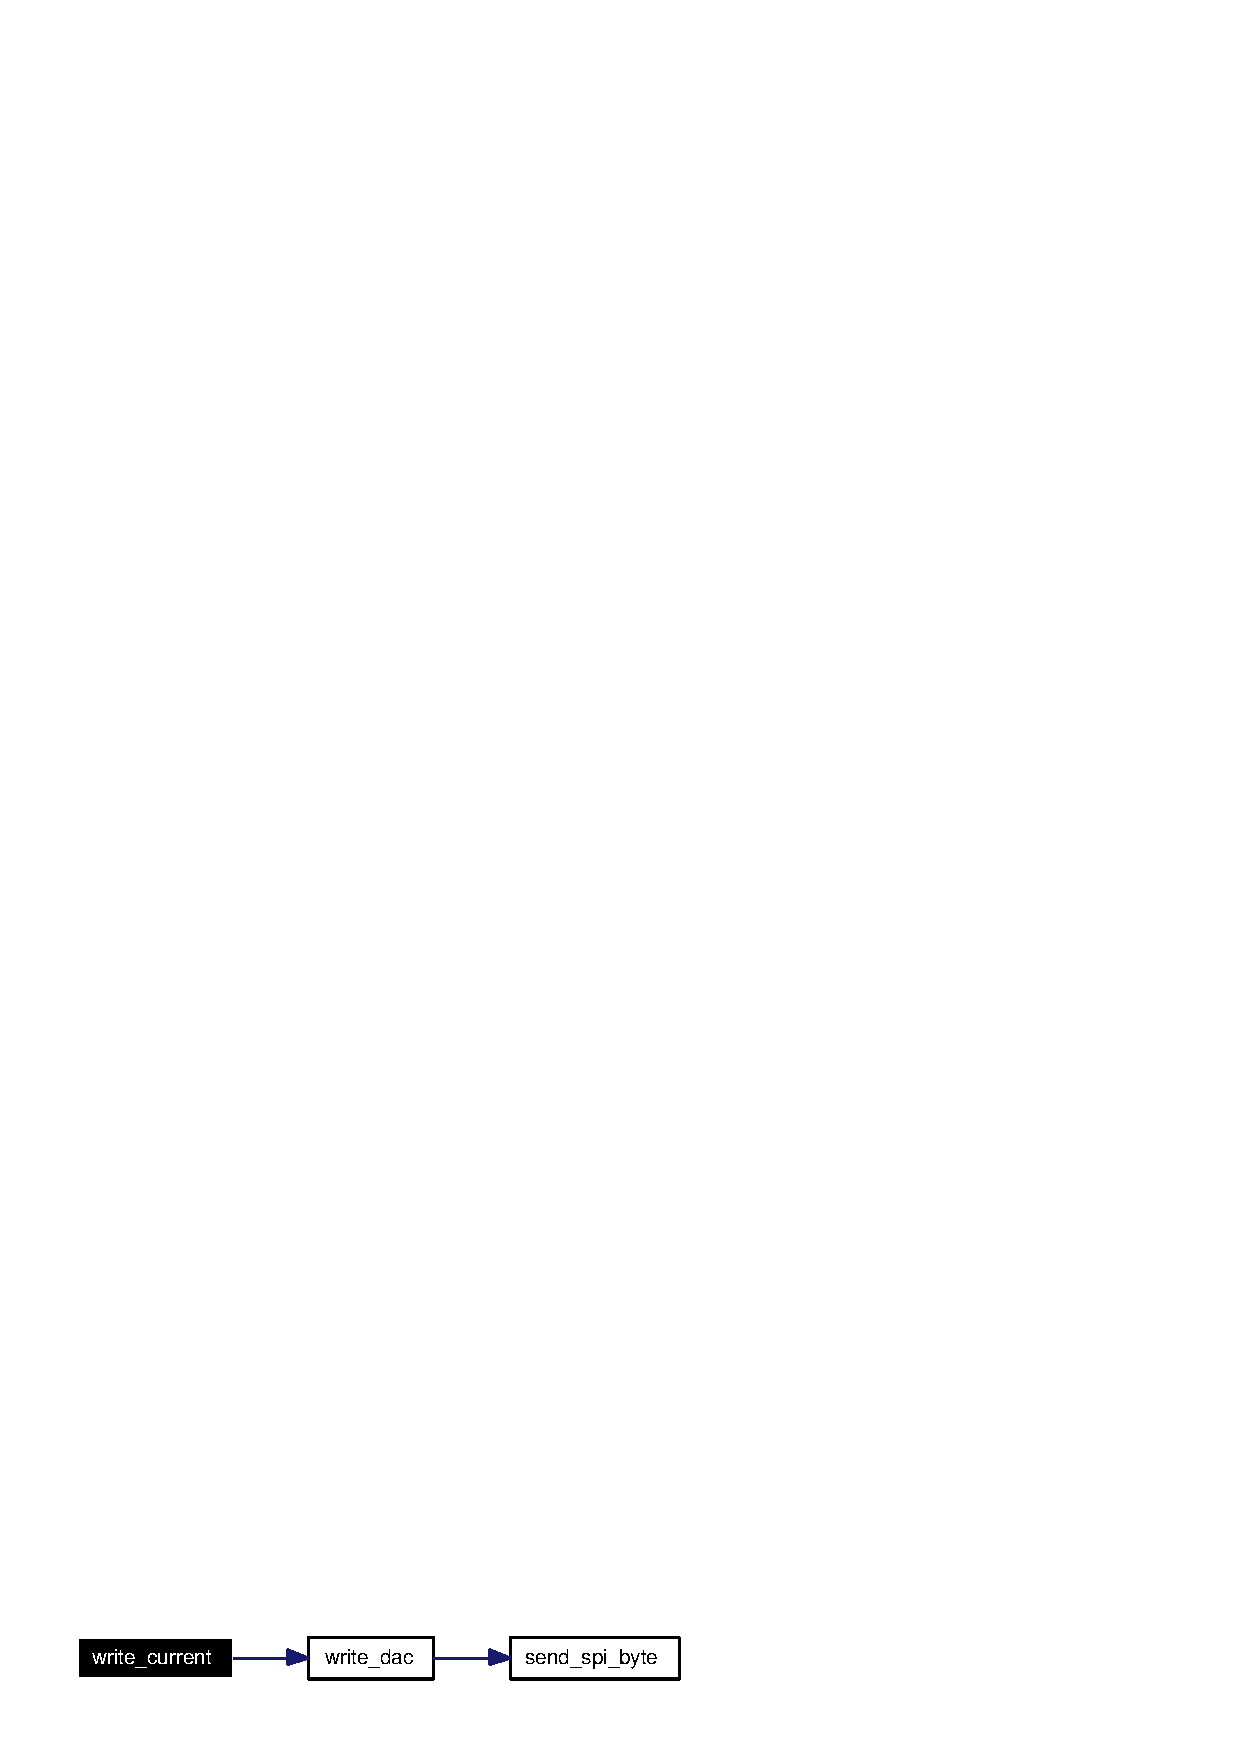
\includegraphics[width=163pt]{ueaclib_8h_a13_cgraph}
\end{center}
\end{figure}
\index{ueaclib.h@{ueaclib.h}!write_dac@{write\_\-dac}}
\index{write_dac@{write\_\-dac}!ueaclib.h@{ueaclib.h}}
\subsubsection{\setlength{\rightskip}{0pt plus 5cm}void write\_\-dac (int, int)}\label{ueaclib_8h_a12}




Definition at line 395 of file ueaclib.c.

References send\_\-spi\_\-byte().

Referenced by current\_\-output\_\-calibration(), and write\_\-current().

\footnotesize\begin{verbatim}395                                       {
396   // write_dac(channel,value)
397   // channel = 0-24 where the channels are the control voltages for the current sources. The current 
398   // sources are labeled starting at the top left corner as follows.
399   //  0  1  2  3  4
400   //  5  6  7  8  9
401   // 10 11 12 13 14
402   // 15 16 17 18 19
403   // 20 21 22 23 24
404   //
405   // Value = 0-1023 (10-bit) where the number represents a control voltage that is 0-3.3v. Each bit represents 
406   // a voltage of 3.3v/1023 or 3.22mV. 
407   //
408   // Hardware Note: Channels 0-23 are implemented by external SPI octal dacs (Linear LTC1660 components). Channel 
409   // 24 is implemented using DAC0 on the MSP430 
410   // 
411   // Initial Version BH 11/1/05
412 
413   if (channel < 8) {
414     P4OUT&=~0x01;                                   // assert the proper chip select
415     channel++;                                      // increment the channel number LTC1660 channels run from 1-8   
416   }           
417   else if (channel < 16) {
418     P4OUT&=~0x02;                                   // assert the proper chip select
419     channel-=7;                                     // bring channel number into range 1-8
420   } 
421   else if (channel < 24) {
422     P4OUT&=~0x04;                                   // assert the proper chip select
423     channel-=15;                                    // bring channel number into range 1-8
424   }
425   else if (channel == 24) {
426     DAC12_0DAT=value<<2;                            // Shift up to a 12-bit number and write to the MSP430 DAC0 
427     return;                                         // This is all to do for the MSP430 DAC case, exit...
428   }
429   else {                                            // channel number provided is too large, exit... 
430     return;
431   }
432   value=(value&0x03FF)<<2;                          // mask and shift the value to align properly in the dac sentence
433   channel<<=4;
434   *(((unsigned char *) &value)+1)|=((unsigned char) channel); // "or" in the channel number to the value data
435   send_spi_byte(*(((unsigned char *) &value)+1));             // send the high byte 
436   send_spi_byte(*((unsigned char *) &value));                 // send the high byte 
437   P4OUT|=0x0F;                                                // deassert all of the spi dac chip selects   
438 }
\end{verbatim}\normalsize 




Here is the call graph for this function:\begin{figure}[H]
\begin{center}
\leavevmode
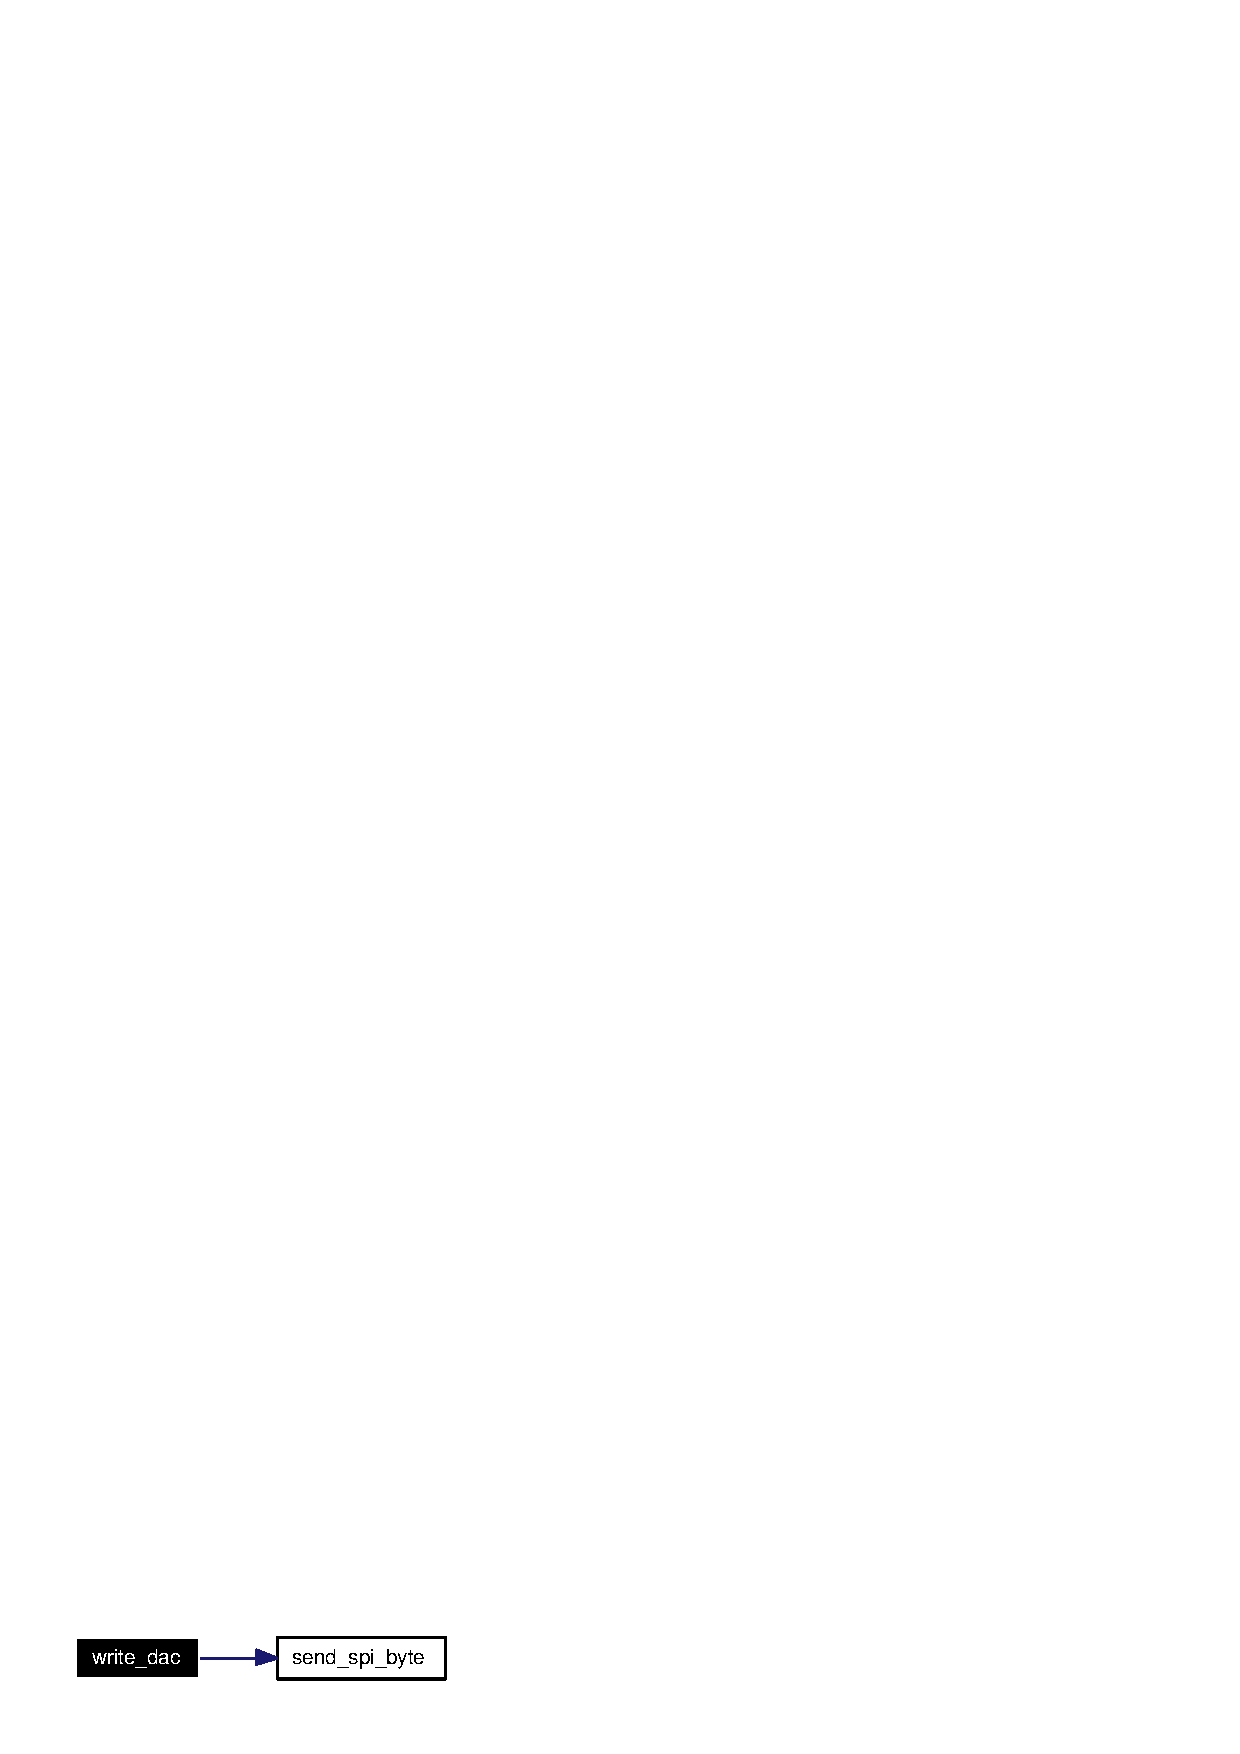
\includegraphics[width=107pt]{ueaclib_8h_a12_cgraph}
\end{center}
\end{figure}
\index{ueaclib.h@{ueaclib.h}!write_led@{write\_\-led}}
\index{write_led@{write\_\-led}!ueaclib.h@{ueaclib.h}}
\subsubsection{\setlength{\rightskip}{0pt plus 5cm}void write\_\-led (int, int)}\label{ueaclib_8h_a14}




Definition at line 497 of file ueaclib.c.

Referenced by current\_\-output\_\-calibration(), main(), and scan\_\-leds().

\footnotesize\begin{verbatim}497                                          {
498   static unsigned long led_state = 0x00000000;
499   if (enable) {
500     if (channel<8) {
501       *((unsigned char *) &led_state) |= 0x01<<channel;       // Save the new state of the LED in led_state
502       P1OUT=*((unsigned char *) &led_state);                  // Place the relevant byte of led_state on the latch bus 
503       P5OUT|=0x01;                                            // strobe the chip select for the target latch
504       P5OUT&=~0x01;                                           // clear the chip select bit
505     }
506     else if (channel<16) {
507       channel-=8;
508       *(((unsigned char *) &led_state)+1) |= 0x01<<channel;  
509       P1OUT=*(((unsigned char *) &led_state)+1);  
510       P5OUT=0x02;
511       P5OUT&=~0x02;                                           // clear the chip select bit
512     }
513     else if (channel<24) {
514       channel-=16;
515       *(((unsigned char *) &led_state)+2) |= 0x01<<channel;  
516       P1OUT=*(((unsigned char *) &led_state)+2);  
517       P5OUT=0x04;
518       P5OUT&=~0x04;                                           // clear the chip select bit
519     }
520     else if (channel==24) {
521       *(((unsigned char *) &led_state)+3) |= 0x01;  
522       P2OUT|=0x01;
523     }
524   }
525   else {
526     if (channel<8) {
527       *((unsigned char *) &led_state) &= ~(0x01<<channel);  
528       P1OUT=*((unsigned char *) &led_state);  
529       P5OUT=0x01;
530       P5OUT&=~0x01;                                           // clear the chip select bit
531     }
532     else if (channel<16) {
533       channel-=8;
534       *(((unsigned char *) &led_state)+1) &= ~(0x01<<channel);  
535       P1OUT=*(((unsigned char *) &led_state)+1);  
536       P5OUT=0x02;
537       P5OUT&=~0x02;                                           // clear the chip select bit
538     }
539     else if (channel<24) {
540       channel-=16;
541       *(((unsigned char *) &led_state)+2) &= ~(0x01<<channel);  
542       P1OUT=*(((unsigned char *) &led_state)+2);  
543       P5OUT=0x04;
544       P5OUT&=~0x04;                                           // clear the chip select bit
545     }
546     else if (channel==24) {
547       *(((unsigned char *) &led_state)+3) &= 0xFE;  
548       P2OUT&=0xFE;
549     }
550   }
551 }
\end{verbatim}\normalsize 


\index{ueaclib.h@{ueaclib.h}!write_lla@{write\_\-lla}}
\index{write_lla@{write\_\-lla}!ueaclib.h@{ueaclib.h}}
\subsubsection{\setlength{\rightskip}{0pt plus 5cm}void write\_\-lla (int, int)}\label{ueaclib_8h_a15}




Definition at line 553 of file ueaclib.c.

Referenced by current\_\-output\_\-calibration(), lla\_\-add(), lla\_\-disable(), lla\_\-enable(), main(), print\_\-grid\_\-i(), and scan\_\-probes().

\footnotesize\begin{verbatim}553                                          {
554   static unsigned long lla_state = 0x00000000;
555   if (enable) {
556     if (channel<8) {
557       *((unsigned char *) &lla_state) |= 0x01<<channel;       // Save the new state of the LED in lla_state
558       P1OUT=*((unsigned char *) &lla_state);                  // Place the relevant byte of lla_state on the latch bus 
559       P5OUT|=0x08;                                            // strobe the chip select for the target latch
560       P5OUT&=~0x08;                                           // clear the chip select bit
561     }
562     else if (channel<16) {
563       channel-=8;
564       *(((unsigned char *) &lla_state)+1) |= 0x01<<channel;  
565       P1OUT=*(((unsigned char *) &lla_state)+1);  
566       P5OUT=0x10;
567       P5OUT&=~0x10;                                           // clear the chip select bit
568     }
569     else if (channel<24) {
570       channel-=16;
571       *(((unsigned char *) &lla_state)+2) |= 0x01<<channel;  
572       P1OUT=*(((unsigned char *) &lla_state)+2);  
573       P5OUT=0x20;
574       P5OUT&=~0x20;                                           // clear the chip select bit
575     }
576     else if (channel==24) {
577       *(((unsigned char *) &lla_state)+3) |= 0x01;  
578       P2OUT|=0x02;
579     }
580   }
581   else {
582     if (channel<8) {
583       *((unsigned char *) &lla_state) &= ~(0x01<<channel);  
584       P1OUT=*((unsigned char *) &lla_state);  
585       P5OUT=0x08;
586       P5OUT&=~0x08;                                           // clear the chip select bit
587     }
588     else if (channel<16) {
589       channel-=8;
590       *(((unsigned char *) &lla_state)+1) &= ~(0x01<<channel);  
591       P1OUT=*(((unsigned char *) &lla_state)+1);  
592       P5OUT=0x10;
593       P5OUT&=~0x10;                                           // clear the chip select bit
594     }
595     else if (channel<24) {
596       channel-=16;
597       *(((unsigned char *) &lla_state)+2) &= ~(0x01<<channel);  
598       P1OUT=*(((unsigned char *) &lla_state)+2);  
599       P5OUT=0x20;
600       P5OUT&=~0x20;                                           // clear the chip select bit
601     }
602     else if (channel==24) {
603       *(((unsigned char *) &lla_state)+3) &= 0xFE;  
604       P2OUT&=0xFD;
605     }
606   }
607 }
\end{verbatim}\normalsize 


